% This file allows to produce either a separate PDF/PNG image
% See standalone documentation to understand underlying magic

\documentclass[tikz,convert={density=150,size=600,outext=.png}]{standalone}
\usetikzlibrary{shapes, calc, arrows, fit, positioning, decorations, patterns, decorations.pathreplacing, chains, snakes}
% Copyright (c) 2016 Grigory Rechistov <grigory.rechistov@phystech.edu>
% This work is licensed under the Creative Commons Attribution-NonCommercial-ShareAlike 4.0 Worldwide.
% To view a copy of this license, visit http://creativecommons.org/licenses/by-nc-sa/4.0/.

\usepackage{fontspec}
\usepackage{xunicode} % some extra unicode support
\usepackage{xltxtra}

\usepackage{amsfonts}
\usepackage{amsmath}
\usepackage{longtable}
\usepackage{csquotes}

\usepackage{polyglossia}
\setdefaultlanguage[spelling=modern]{russian} % for polyglossia
\setotherlanguage{english} % for polyglossia

% Common settings for all fonts
% 1. Attempt to make fonts be of the same size
% 2. Support TeX ligatures like — = emdash, << >> = guillemets
\defaultfontfeatures{Scale=MatchLowercase, Mapping=tex-text}

% Use Computer Modern Unicode
\newfontfamily\russianfont{CMU Serif}
\setromanfont{CMU Serif}
\setsansfont{CMU Sans Serif}
\setmonofont{CMU Typewriter Text}

% Copyright (c) 2016 Grigory Rechistov <grigory.rechistov@phystech.edu>
% This work is licensed under the Creative Commons Attribution-NonCommercial-ShareAlike 4.0 Worldwide.
% To view a copy of this license, visit http://creativecommons.org/licenses/by-nc-sa/4.0/.

% Common packages, commands and their configuration

\newcommand{\abbr}{\textit{англ.}\ }
\newcommand{\todo}[1][]{\textcolor{red}{TODO #1}}

\usepackage{graphicx}
\graphicspath{{pictures/}} % path to pictures, trailing slash is mandatory.

\usepackage{hyperref}
\hypersetup{colorlinks=true, linkcolor=black, filecolor=black, citecolor=black, urlcolor=black , pdfauthor=Grigory Rechistov <grigory.rechistov@phystech.edu>, pdftitle=Программное моделирование вычислительных систем}

\usepackage{footnpag}
\usepackage{indentfirst}
\usepackage{underscore}
\usepackage{url}

\usepackage{listings}
\lstset{basicstyle=\footnotesize\ttfamily, breaklines=true, keepspaces=true }

\usepackage{tikz}
\usetikzlibrary{shapes, calc, arrows, fit, positioning, decorations, patterns, decorations.pathreplacing, chains, snakes}
\usepackage{bytefield}

\usepackage{pgfplots} % Draw plots inside TeX
\pgfplotsset{compat=1.10}

\usepackage{standalone} % Clever way to build TikZ pictures either to PDF or to PNG


\graphicspath{{../pictures/}} % path to pictures, trailing slash is mandatory.

% The actual drawing follows
\begin{document}
\begin{tikzpicture}[>=latex, font=\small, node distance=0.3cm, inner sep=0pt]
    
    \node (tower) {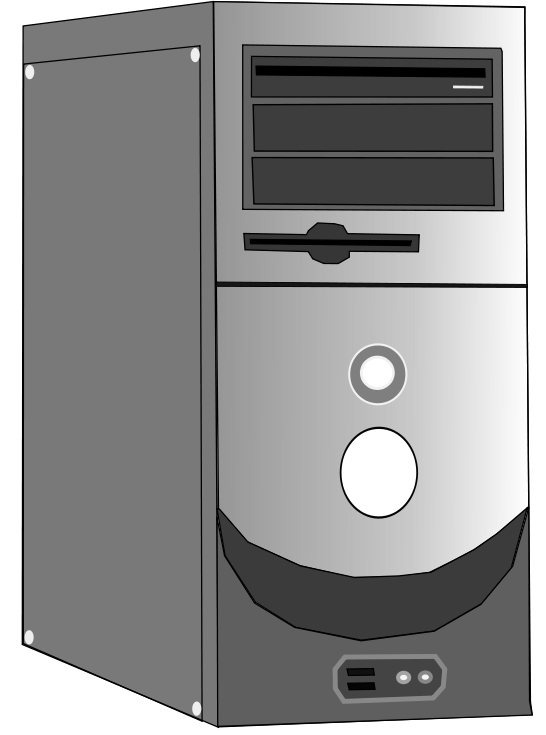
\includegraphics[height=1.5cm]{./tower.png}};
    \node[above=of tower] (monitor1) {
\includegraphics[height=1.2cm]{./monitor1.png}};
    \node[right =0.2cm of monitor1] (kb1) {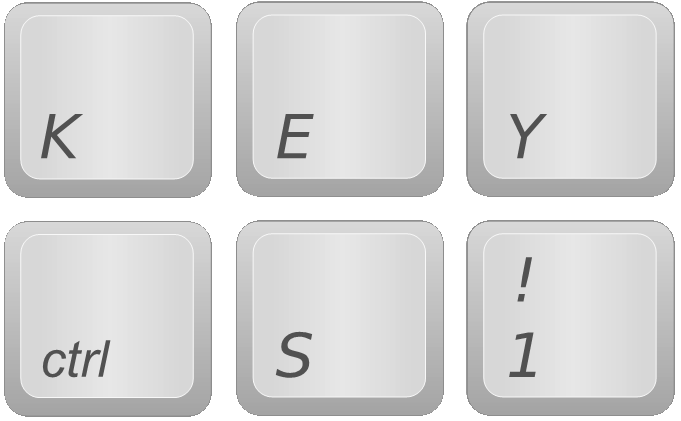
\includegraphics[height=.8cm]{./kb1.png}};
    
    % Inner border
    \node[draw, inner sep=0.2cm, fit=(tower) (monitor1) (kb1)] (virt) {};
    
    \node[right =2.cm of tower] (folder) {
\includegraphics[height=1.cm]{./folder.png}};
    \node[right =0.2cm of folder] (hdd) {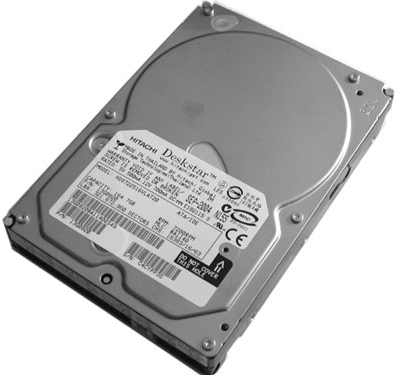
\includegraphics[height=1.cm]{./device3.png}};
    
    \node[right=0.7cm of hdd] (stub) {};
    
    % The outer border
    \node[draw, inner sep=0.35cm, fit= (virt) (tower) (monitor1) (kb1)  (hdd) (stub)]  (real) {};
    
    \node[right =0.2cm of hdd] (nic) {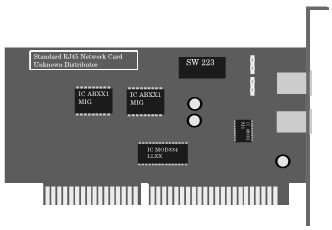
\includegraphics[height=1.cm]{./nic.png}};
    \node[right =of kb1, yshift=1cm] (kb2) {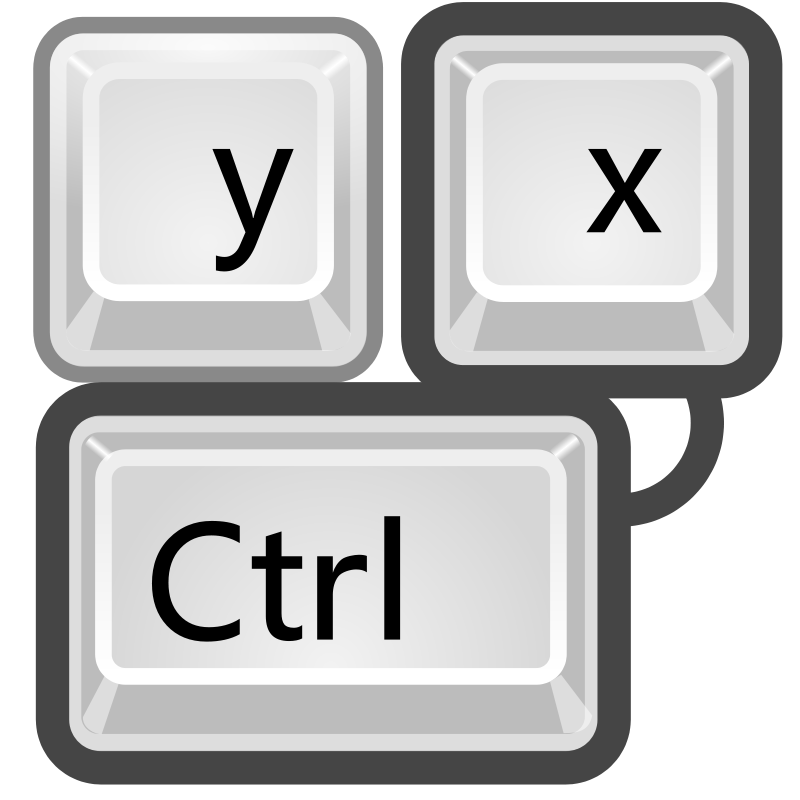
\includegraphics[height=1.5cm]{./kb2.png}};
    \node[right =of kb2] (monitor2) {
\includegraphics[height=1.5cm]{./monitor2.png}};   
    
    \node[fill=white, font=\scriptsize] at (virt.south) {Граница ВМ};
    
    \node[fill=white, font=\scriptsize] at (real.south) {Граница реальной системы};
\end{tikzpicture}


\end{document}
